\documentclass[a4paper,11pt]{article}
\usepackage[english]{babel}
\usepackage[utf8]{inputenc}
\usepackage[T1]{fontenc}
\usepackage[a4paper,margin=1.5cm,top=1.2cm,bottom=1.2cm]{geometry}
\usepackage{graphicx}
\usepackage{amsmath}
\usepackage{booktabs}
\usepackage{siunitx}
\usepackage{float}
\usepackage{microtype}
\usepackage{newtxtext,newtxmath}
\usepackage{setspace}
\usepackage{fancyhdr}
\usepackage{longtable}
\setstretch{1.15}

\pagestyle{fancy}
\fancyhf{}
\fancyfoot[C]{\thepage}
\renewcommand{\headrulewidth}{0pt}
\renewcommand{\footrulewidth}{0pt}
\setlength{\headheight}{14pt}
\setlength{\footskip}{14pt}

\begin{document}

\title{M33. Interferences in the Quincke Tube}
\author{Andrés Vinuesa Espinosa}
\maketitle

\begin{abstract}
This report investigates the phenomenon of acoustic interference using a Quincke tube. By measuring the transmitted sound intensity as a function of both frequency and path length difference, constructive and destructive interference patterns were identified. These observations were used to determine the speed of sound and the characteristic length of the apparatus. The experimental results for the speed of sound were compared with theoretical values calculated from the ambient temperature.
\end{abstract}

\section{Introduction and Objectives}

\subsection{Objectives}
\begin{itemize}
    \item Verify the occurrence of constructive and destructive interference in sound waves.
    \item Determine the speed of sound through the analysis of interference patterns.
    \item Calculate the characteristic length of the Quincke tube.
\end{itemize}

\subsection{Theoretical Background}
Interference occurs when two or more waves coincide in space and time. In a Quincke tube, a pressure wave from a source is split into two paths of lengths $a$ and $b$. These waves interfere at a receiver. The path difference is given by:
\begin{equation}
    b - a = 2\Delta d
\end{equation}
where $\Delta d$ is the displacement of the movable arm. The condition for constructive interference (maxima) and destructive interference (minima) is:
\begin{equation}
    \Delta d = n \frac{c}{4f}
\end{equation}
where $n$ is a relative ordinal, $c$ is the speed of sound, and $f$ is the frequency. When the paths are equal ($a=b$), resonance frequencies can occur according to:
\begin{equation}
    f_n = n \frac{c}{2a}
\end{equation}

\section{Materials and Methods}

\subsection{Experimental Setup}
The setup includes a Quincke tube with a movable arm, a speaker as a sound source connected to a function generator, and a microphone connected to a voltmeter or oscilloscope.

\subsection{Data Acquisition and Analysis}
Two main experiments were performed:
\begin{enumerate}
    \item \textbf{Experiment A/B}: Frequencies corresponding to maxima and minima were identified for a fixed tube configuration ($a \approx b$).
    \item \textbf{Experiment C}: The sound amplitude (voltage) was recorded as a function of the arm displacement $\Delta d$ for a fixed frequency $f = 1576$ Hz.
\end{enumerate}
The speed of sound $c$ was determined by fitting the positions of maxima and minima in Experiment C to the linear relation $\Delta d(n)$.

\section{Results and Data Analysis}

\subsection{Voltage vs Frequency}
The experimental results for the transmitted sound intensity as a function of frequency are displayed in Figure \ref{fig:v_vs_f}.

\begin{figure}[H]
    \centering
    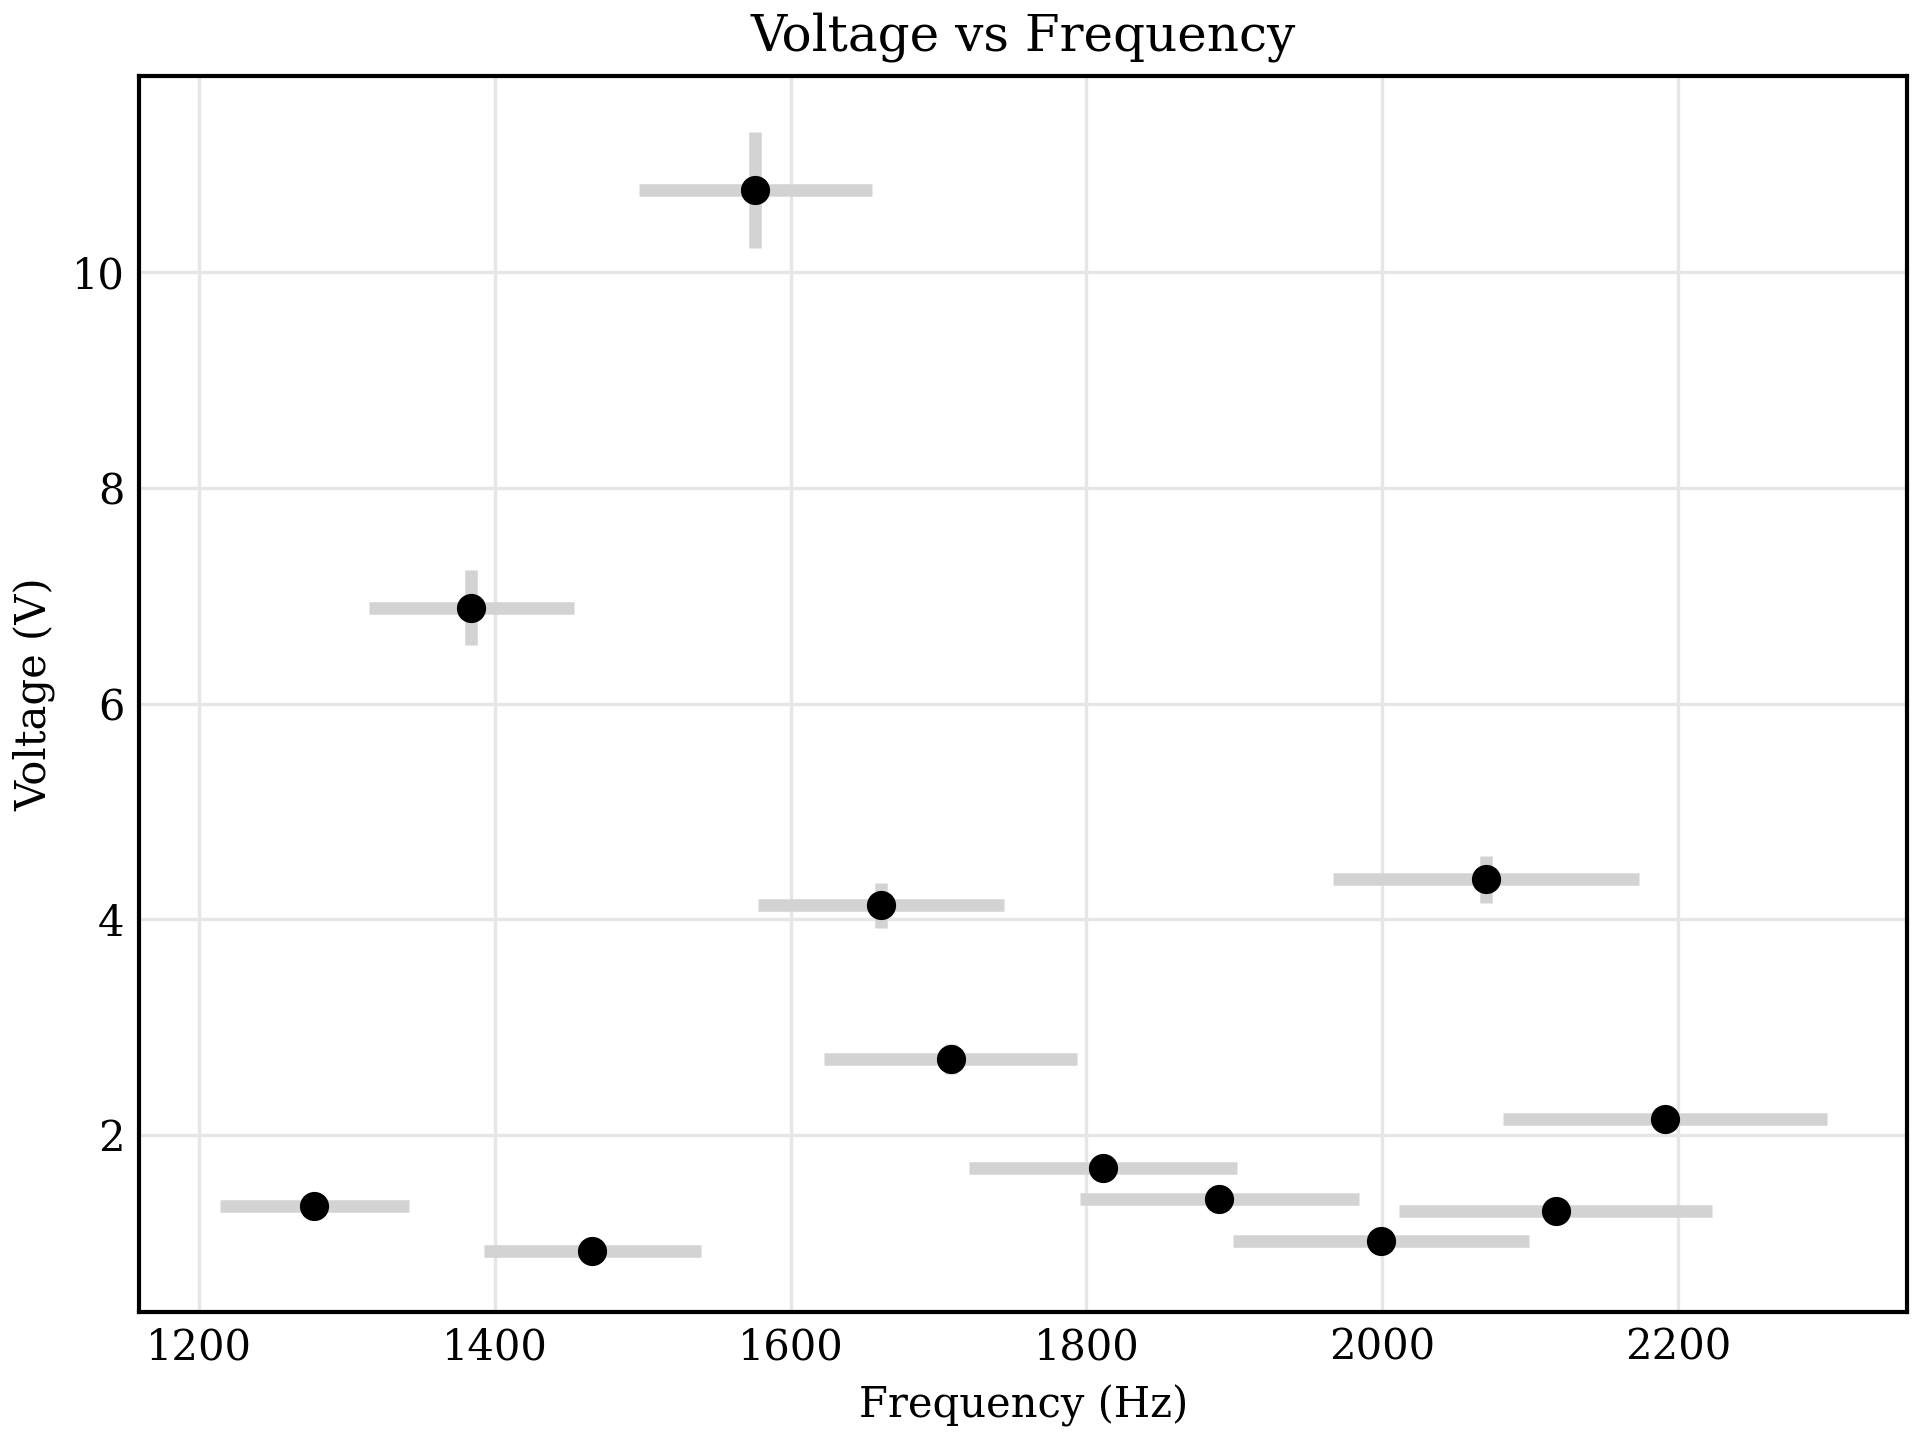
\includegraphics[width=0.8\textwidth]{m33_voltaje_vs_frecuencia.png}
    \caption{Sound amplitude (Voltage) as a function of source frequency.}
    \label{fig:v_vs_f}
\end{figure}

\subsection{Voltage vs Distance}
For a fixed frequency $f = 1576$ Hz, the voltage was measured as the arm displacement $\Delta d$ was varied. The resulting interference pattern is shown in Figure \ref{fig:v_vs_d_plot}.

\begin{figure}[H]
    \centering
    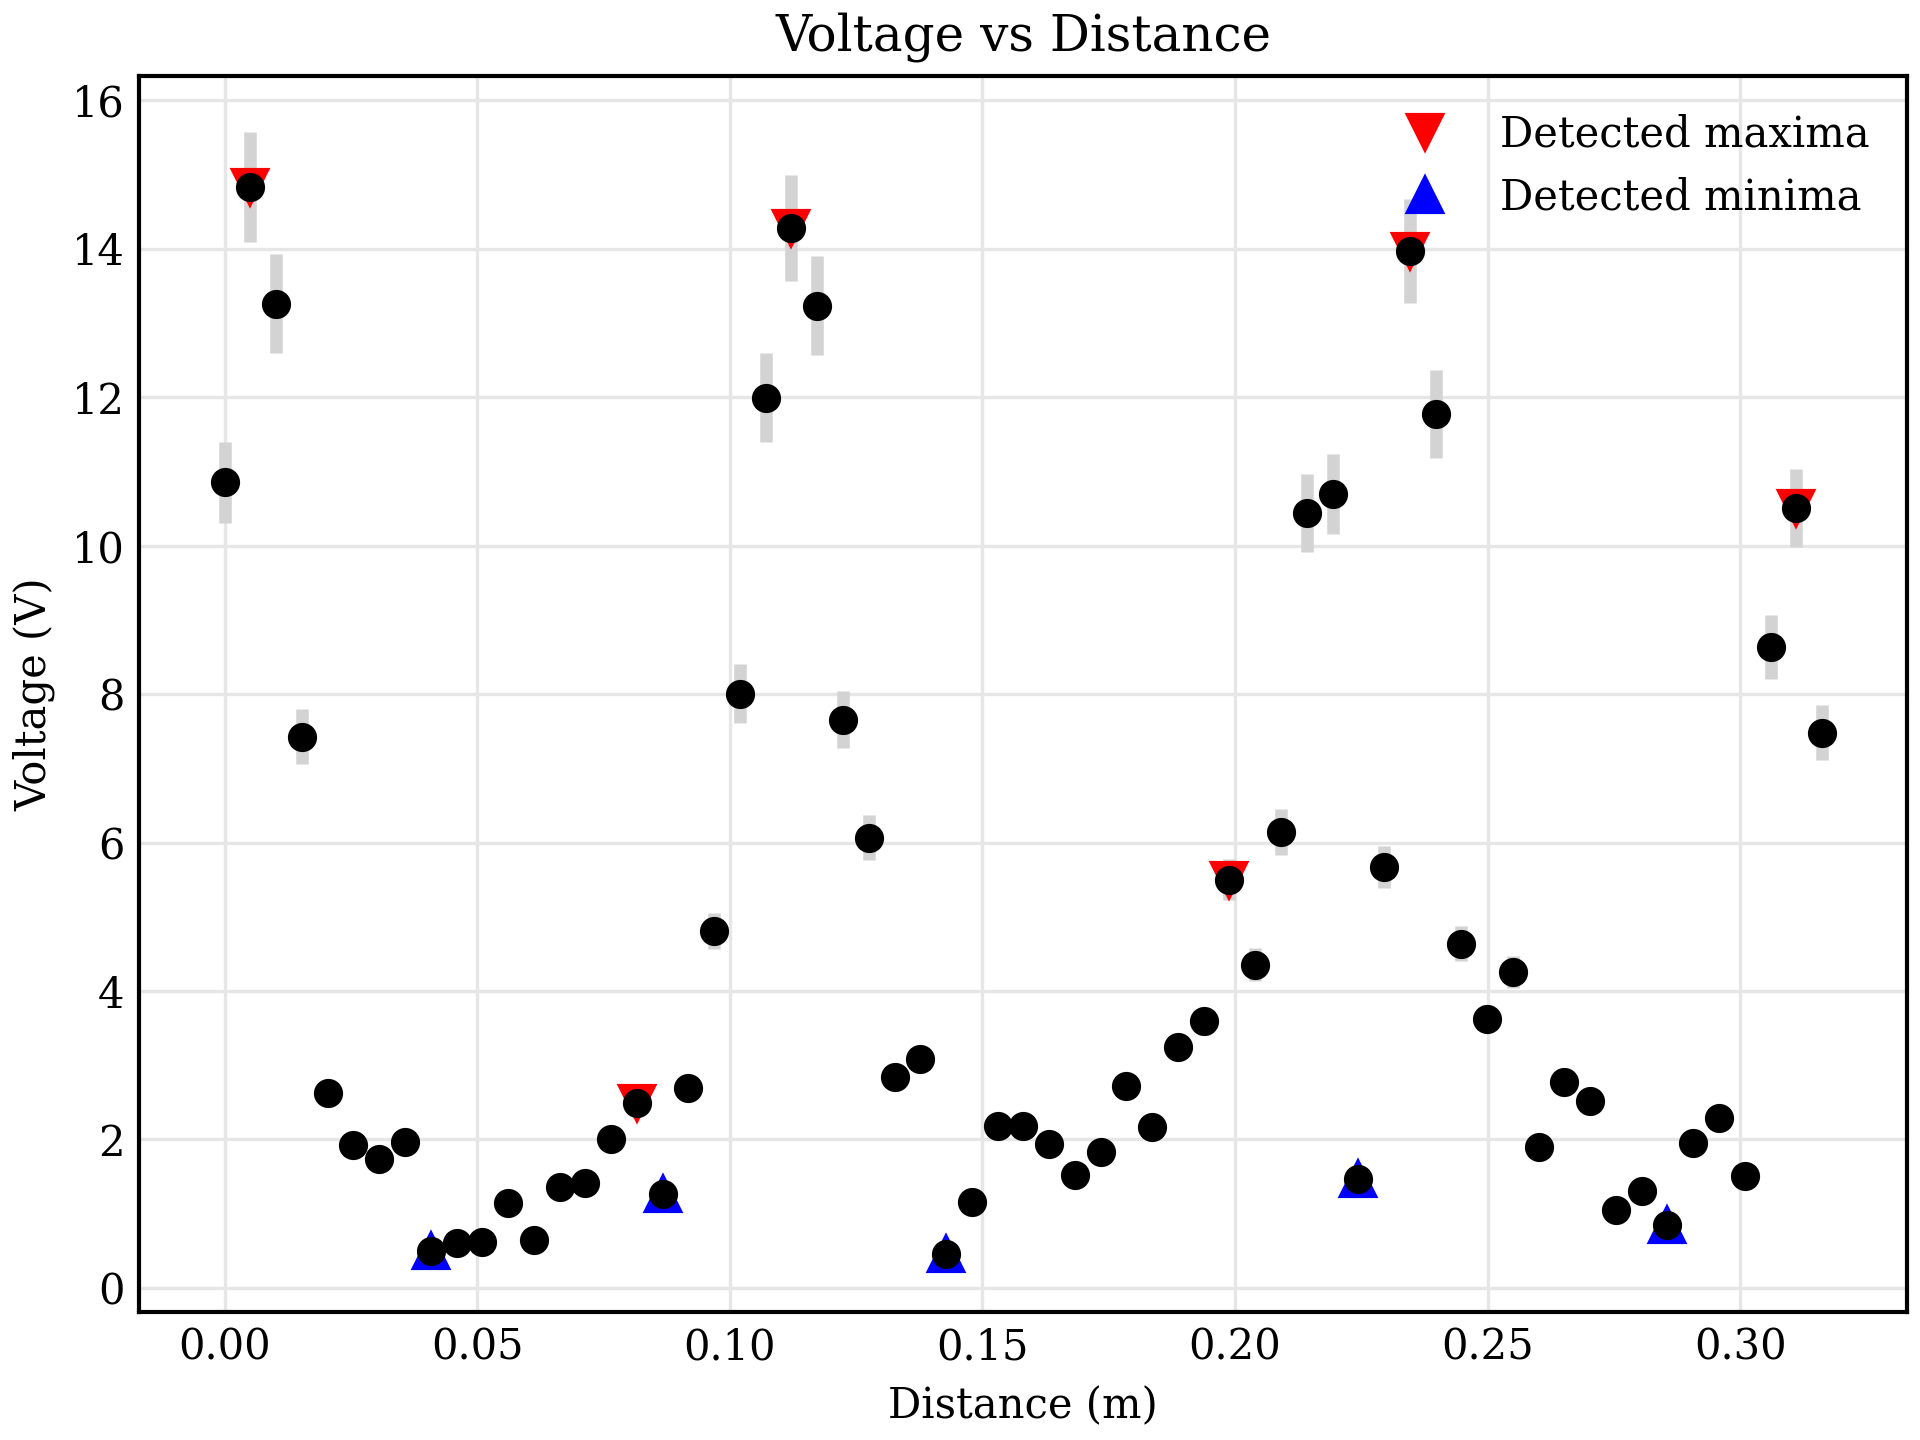
\includegraphics[width=0.8\textwidth]{m33_voltaje_vs_distancia.png}
    \caption{Sound amplitude (Voltage) as a function of movable arm displacement $\Delta d$.}
    \label{fig:v_vs_d_plot}
\end{figure}

\subsection{Determination of Sound Speed}
The detected peaks (maxima) and troughs (minima) from Experiment C were used to perform a linear fit of $\Delta d$ vs $n$.

\begin{figure}[H]
    \centering
    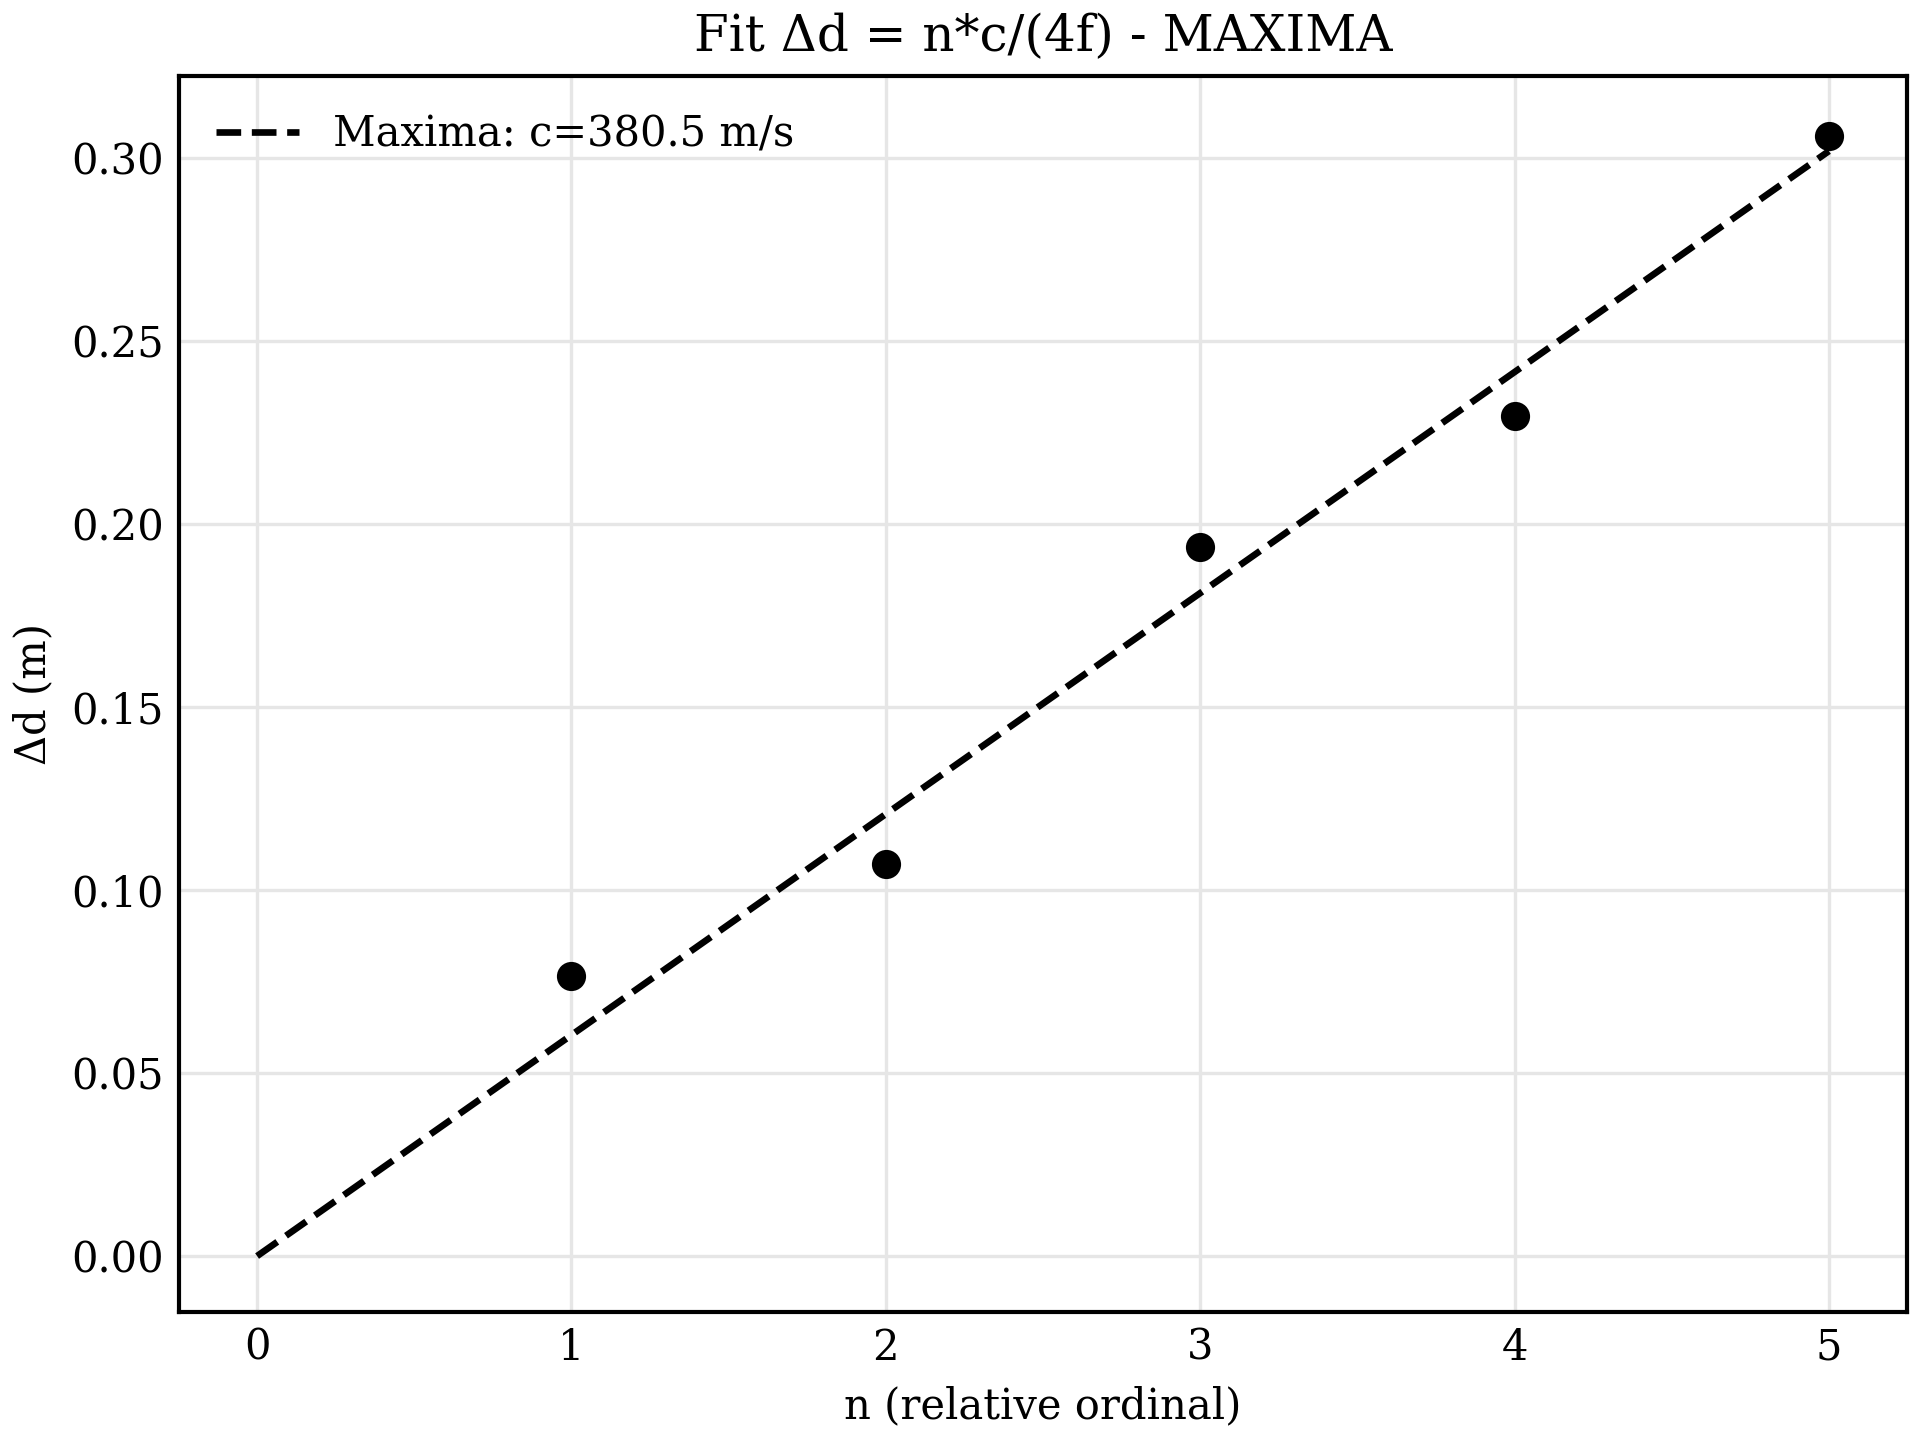
\includegraphics[width=0.45\textwidth]{m33_ajuste_maximos.png}
    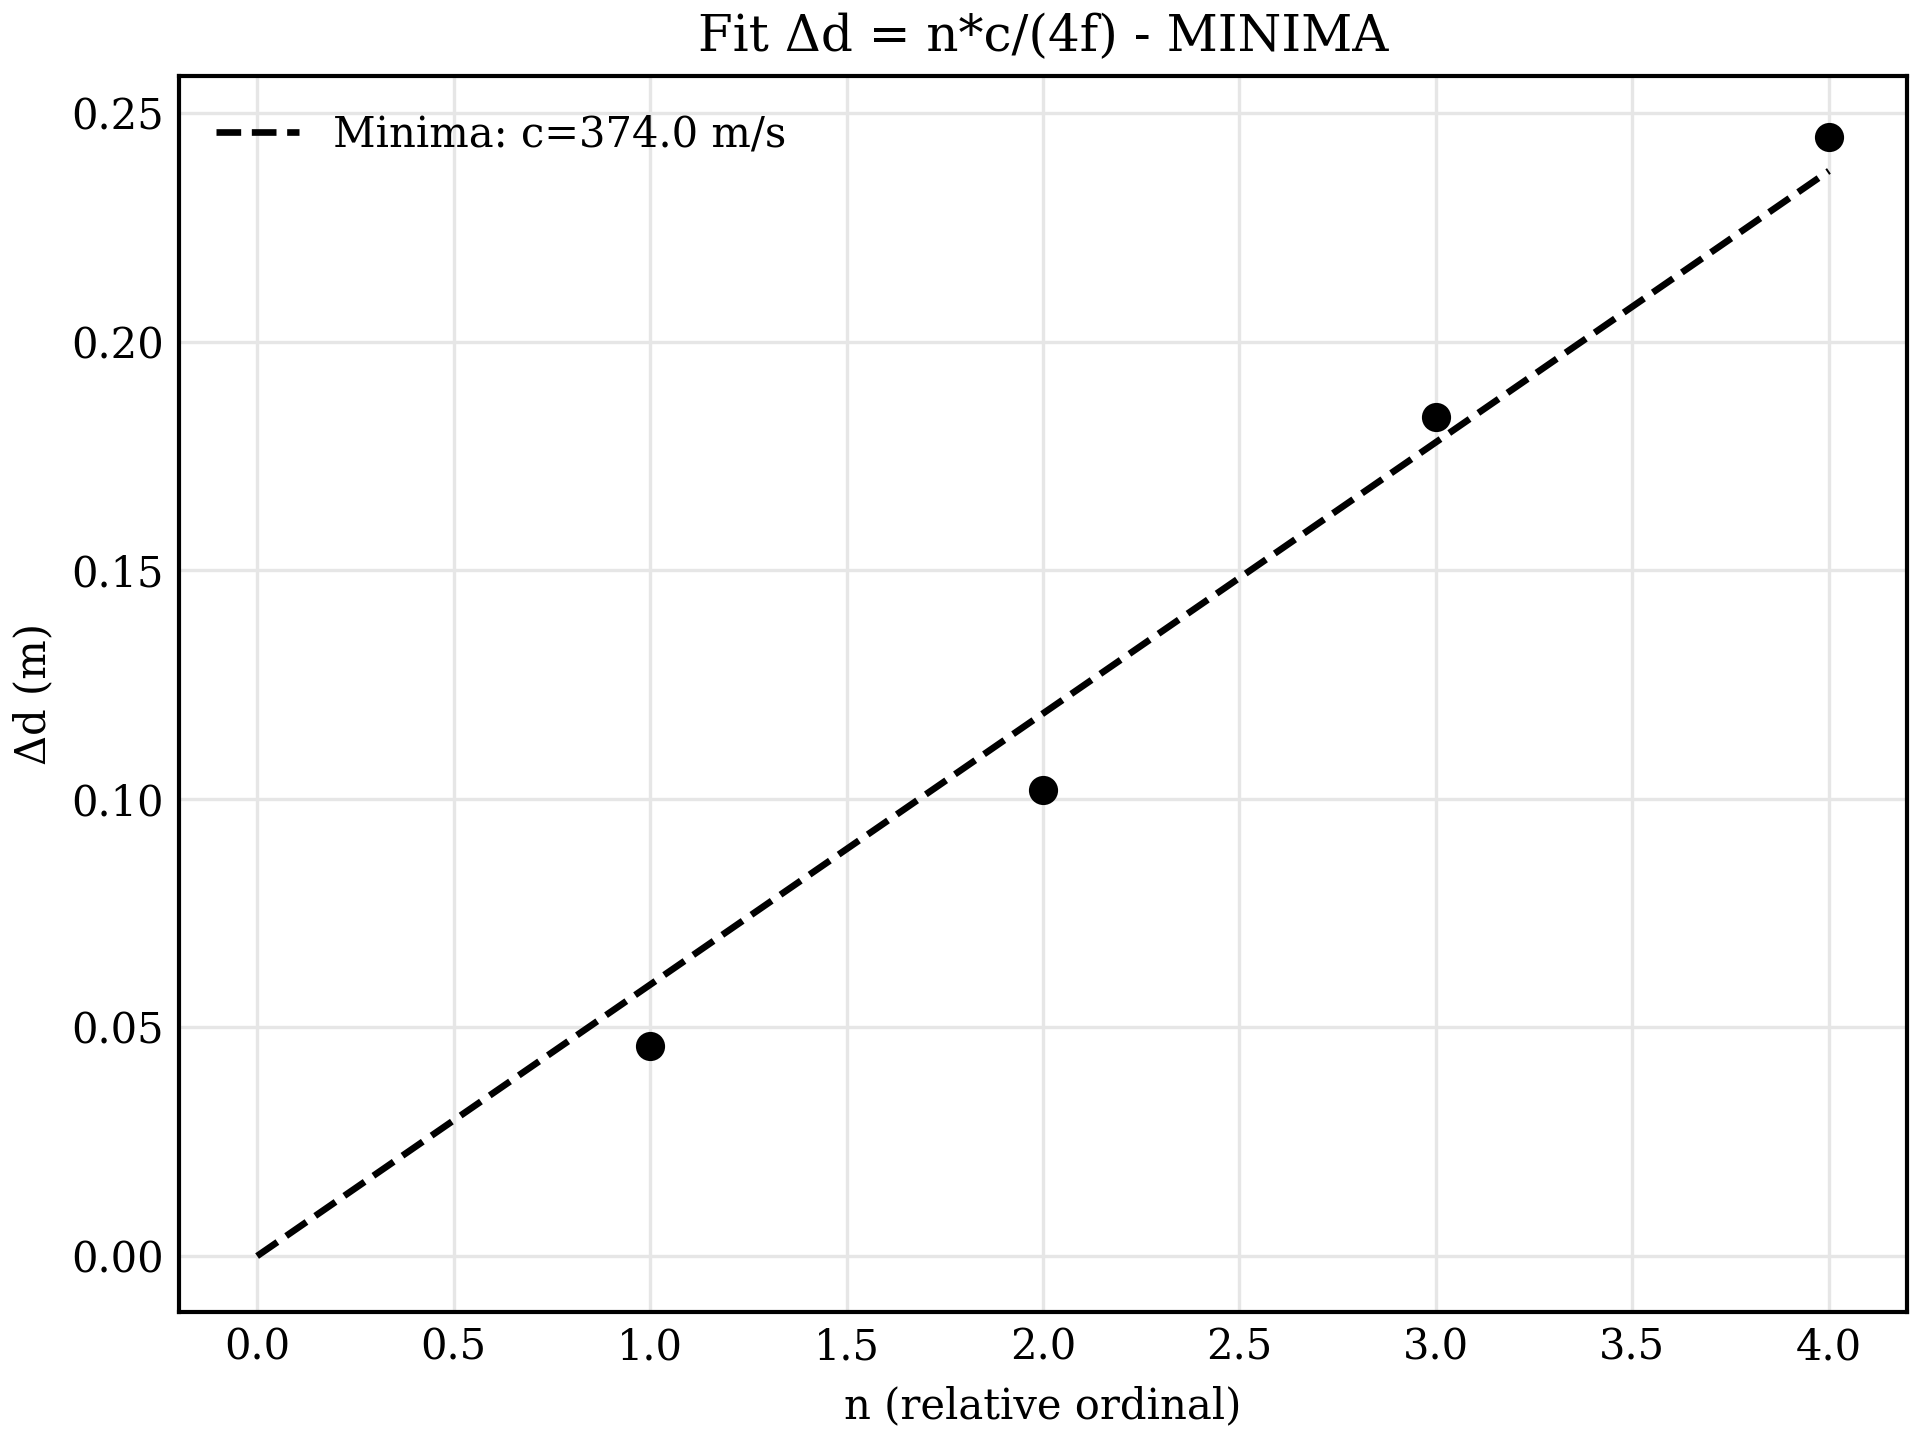
\includegraphics[width=0.45\textwidth]{m33_ajuste_minimos.png}
    \caption{Linear fits for sound speed determination using maxima (left) and minima (right).}
    \label{fig:fits}
\end{figure}

The resulting values for the speed of sound are:
\begin{itemize}
    \item \textbf{From Maxima}: $c = \qty{380.54 \pm 0.85}{\unit{m/s}}$
    \item \textbf{From Minima}: $c = \qty{374.02 \pm 1.2}{\unit{m/s}}$
\end{itemize}

The theoretical speed of sound at $\theta = \qty{27.5}{^\circ C}$ (equivalent to $T = \qty{300.65}{K}$) is calculated as:
\begin{equation}
    c_{theory} = 331.3 \sqrt{1 + \frac{\theta}{273.15}} = 331.3 \sqrt{\frac{300.65}{273.15}} = \qty{347.58}{\unit{m/s}}
\end{equation}

The relative differences between the experimental and theoretical values are:
\begin{itemize}
    \item \textbf{Maxima}: 9.48 \%
    \item \textbf{Minima}: 7.61 \%
\end{itemize}

\section{Discussion and Conclusions}
% [HUMAN AUTHOR: WRITE DISCUSSION/CONCLUSIONS HERE]

\appendix
\section{Uncertainty Analysis}
The uncertainty in voltage $u_V$ was calculated as $5\%$ of the reading plus an instrumental offset of $0.001 \unit{V}$. The uncertainty in frequency $u_f$ was estimated as $5\%$ of the set value. For the distance $\Delta d$, a fixed uncertainty of $0.1 \unit{cm}$ was assumed based on the scale of the movable arm. The uncertainty in the fitted speed of sound was derived from the variance of the weighted linear fit through the origin.

\end{document}